\documentclass[10.5pt,a4paper]{article}

% Packages for formatting and layout
\usepackage{geometry}  % Adjust margins
\geometry{margin=0.5in}
\usepackage{setspace}  % For line spacing
\usepackage{graphicx, wrapfig}
\graphicspath{ {./assets/} }
\usepackage{amsmath}   % For mathematical expressions
\usepackage{hyperref}  % For hyperlinks
\usepackage{enumitem}  % For custom lists
\usepackage{listings}
\usepackage{subcaption}
\usepackage{xcolor}
\usepackage{comment}
\usepackage{subcaption}
\renewcommand{\thesubfigure}{\arabic{subfigure}}


\definecolor{codegreen}{rgb}{0,0.6,0}
\definecolor{codegray}{rgb}{0.5,0.5,0.5}
\definecolor{codepurple}{rgb}{0.58,0,0.82}
\definecolor{backcolour}{rgb}{0.95,0.95,0.92}

\lstdefinestyle{mystyle}{
    backgroundcolor=\color{backcolour},   
    commentstyle=\color{codegreen},
    keywordstyle=\color{magenta},
    numberstyle=\tiny\color{codegray},
    stringstyle=\color{codepurple},
    basicstyle=\ttfamily\footnotesize,
    breakatwhitespace=false,         
    breaklines=true,                 
    captionpos=b,                    
    keepspaces=true,                 
    numbers=left,                    
    numbersep=5pt,                  
    showspaces=false,                
    showstringspaces=false,
    showtabs=false,                  
    tabsize=2
}

\lstset{style=mystyle}

% Title information
\title{Computer Vision Mid-Term Project}
\author{Baggio Davide 2122547 \\ Martinez Zoren 2123873 \\ Pivotto Francesco 2158296}
\date{}

\usepackage{etoolbox}
\makeatletter
\patchcmd{\@maketitle}{\null\vskip 2em}{}{}{}
\makeatother

\begin{document}

% Title Page
\maketitle

\section*{Introduction}

The goal of this project was to develop, using exclusively the \texttt{OpenCV} library, a detection system capable of locating and delimiting known instances of three objects in input images by means of a bounding box.
\\\\
For object recognition (sugar box, mustard bottle, and power drill), a subset of the public \textbf{YCB Video} dataset was used, which provides for each object:
a \textbf{test\_images} folder containing the test images; a \textbf{models} folder with 60 different views and the corresponding binary segmentation masks; a \textbf{labels} folder containing ground truth annotations for object localization.

\\

\section*{Methodology}

For object detection and localization, we implemented and compared three different methods: Haar Cascades, SIFT-based matching, and ORB-based matching. We independently implemented the three methods and combined their results. Each method returns a set of \textbf{keypoints} representing the features points of the objects we are trying to detect. Below are some additional details on how we implemented each of the three detectors.

\subsubsection*{Haar Cascade Classifer}
    Cascade classifiers in OpenCV, such as Haar cascades, are trained using a sequence of increasingly complex stages. Each stage uses simple features (Haar-like features) extracted from images. Haar features are rectangular regions over which pixel intensity sums are computed quickly via an integral image. The difference between these sums (such as the difference between a bright and dark region) captures characteristic patterns like edges, lines, and center-surround contrasts.

    Training a custom Haar cascade is done using the \texttt{opencv\_traincascade} tool. A typical training command is:

    \begin{lstlisting}[]
opencv_traincascade -data object_cascade -vec positives.vec -bg negative.txt -numPos 29 -numNeg 100 -w 24 -h 24 -maxFalseAlarmRate 0.3 -minHitRate 0.999 -numStages 8
    \end{lstlisting}

    Here, \texttt{-data} specifies the output directory, \texttt{-vec} provides positive samples, \texttt{-bg} lists negative images, and other parameters control training size and complexity.

\subsubsection*{ORB-Based Feature Matching}
    Initially it calculates and stores the feature descriptors of the object models. These descriptors are then used to compare with those of the test image using a \textbf{BFMatcher with Hamming distance} to find matches. For each searched object, the model with the most matches to the test image is considered the best, and the corresponding keypoints are returned for object identification. Finally, the keypoints are ranked based on the distance between the image descriptors and the test descriptors. This ensures that the best keypoints are ordered and can be filtered according to the \textbf{specified percentage}. The \textbf{default parameters} were kept for the initial ORB configuration. This decision was made because we tested several parameter values but did not observe any significant improvement in performance.

\subsubsection*{SIFT-Based Feature Matching}
    During the creation of the detector, the feature descriptors for all object models are computed and stored.\\
    The test image is then preprocessed by converting it to grayscale and applying histogram equalization, which is also performed on the model images to ensure consistency.\\
    Next, matches between the feature descriptors of the test image and those of the models are computed using a \textbf{BFMatcher} with \textbf{KNN matching}. To reduce false positives, the \textbf{Lowe’s Ratio test} is applied.\\
    For each object, the model with the most matches is selected, and the corresponding keypoints are returned for identification. Finally, the keypoints are ranked based on the distance between the image and model descriptors, ensuring the best keypoints are ordered and can be filtered based on the specified percentage.

\subsubsection*{Keypoint Aggregation}
The keypoints identified by the different methods were grouped together. Given the abundance of false positives in many object features, and the fact that the three methods produced an unbalanced number of keypoints, we decided to apply a percentage threshold for each method to filter their output keypoints. We conducted several experiments on the percentage thresholds and ultimately selected the configuration that gave the best results. We kept the output percentage of the best keypoints as follows: \textbf{50\% from the Haar detector, 100\% from ORB, and 50\% from SIFT}.
The final filtering step was applied based on color information to reduce outliers. For each object, we verify that the keypoints fall on pixels with colors consistent with the known appearance of the object. Keypoints that do not match are discarded.

\subsubsection*{Bounding Box Drawing for Object Identification Using Keypoints}
After applying all the methods already explained, multiple candidate detections often appear, especially in noisy scenes. To localize the most probable area where detections are dense, the DBSCAN (Density-Based Spatial Clustering of Applications with Noise) algorithm can be applied. DBSCAN groups nearby points based on two parameters: \texttt{eps} (maximum neighborhood radius) and \texttt{minPts} (minimum number of points to form a cluster). It identifies clusters of high density without requiring the number of clusters in advance.

The largest cluster obtained by DBSCAN can be bounded by a rectangle, representing the area of maximum detection density. This approach is particularly useful for refining detection results and reducing false positives in crowded scenes.

\section*{Results}
The performance of the system was evaluated using two main metrics:
\begin{itemize}
    \item \textbf{Mean Intersection over Union (mIoU)}: the average IoU computed for each object category. \\The detection system achieved a mean IoU of \textbf{0.266419}.
    \item The number of successfully detected objects: \textbf{9/42}.

\end{itemize}

\section*{Difficulties Encoutered}
During the development phase, several critical issues were encountered.\\
For the ORB detector, a major problem was that the logo printed on the sugar box attracted a large number of keypoints, even when compared against models that were not the sugar box itself. This led to incorrect matches and a high rate of false positives.
\begin{figure}[h]
    \centering
    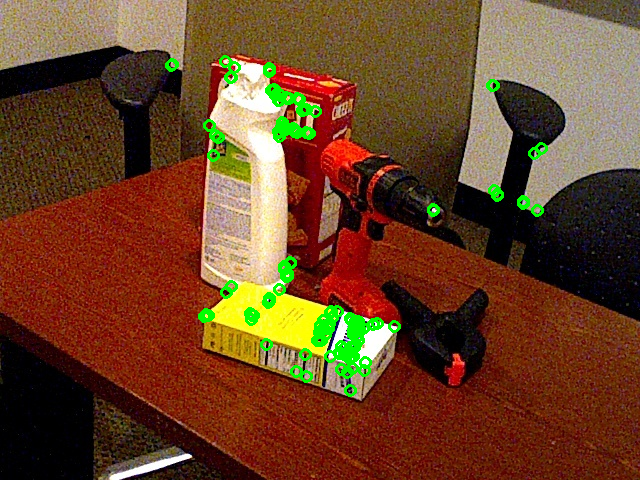
\includegraphics[width=0.3\textwidth]{img/power_drill matches_screenshot_28.04.2025.png}
    \caption{ORB: While searching for the power drill, keypoints are "stolen" by the sugar box.}
    \label{fig:prima}
\end{figure}
\\\\
Regarding the SIFT detector, difficulties were mainly observed in recognizing the mustard bottle and the power drill. In both cases, very few keypoints were detected, and the mustard bottle could only be reliably recognized when seen from a frontal view. On the other hand, the sugar box generally provided a sufficient number of keypoints, but again with a significant number of false matches.
\begin{figure}[h]
    \centering
    \begin{subfigure}{0.3\textwidth}
        \centering
        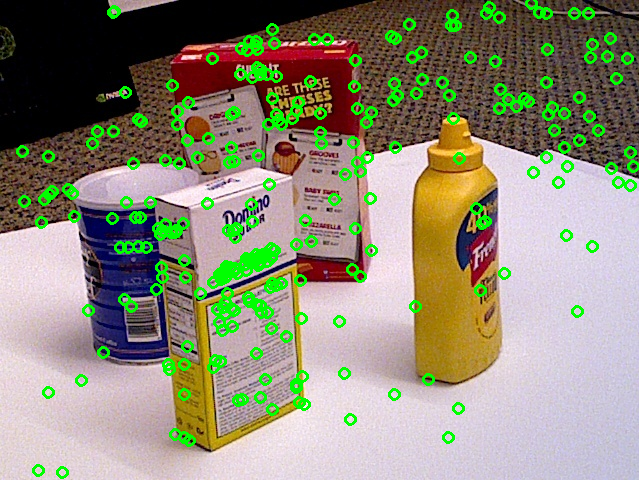
\includegraphics[width=\textwidth]{img/SiFT_PreLowe.png}
        \caption{SIFT: Pre-Lowe}
        \label{fig:PreLowe}
    \end{subfigure}
    \hspace{0.10\textwidth}
    \begin{subfigure}{0.3\textwidth}
        \centering
        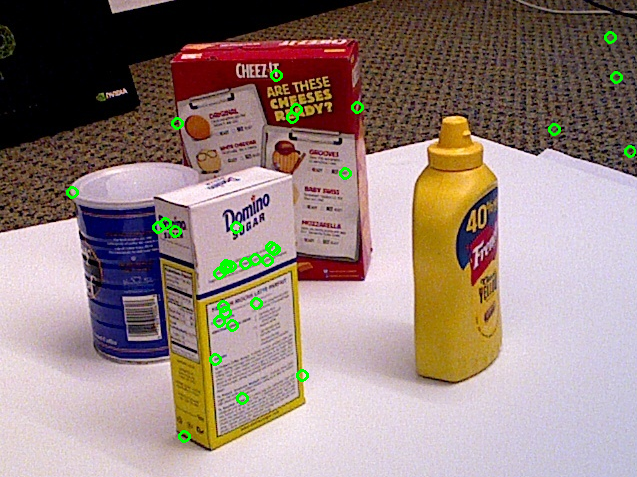
\includegraphics[width=\textwidth]{img/SIFT_PostLowe.png}
        \caption{SIFT: Post-Lowe}
        \label{fig:PostLowe}
    \end{subfigure}
    \caption{Keypoint Matches: Before vs. After Lowe’s Ratio Test}
    \label{fig:confronto}
\end{figure}
\\\\
To address these issues, three different types of filters \textbf{Bilateral}, \textbf{Gaussian}, and \textbf{Median} were tested to improve the quality of the test images. Although they slightly improved the detection performance for the power drill by eliminating some false positives, they significantly blurred the features of the sugar box, drastically reducing the number of detectable keypoints. For this reason, the use of these filters was ultimately discarded.
\\\\
After introducing the Lowe's Ratio Test, which effectively reduced false positives, a further solution was attempted: filtering the keypoints detected by ORB by keeping only those located near the keypoints identified by SIFT. Since SIFT keypoints were more reliable, the goal was to increase the density of ORB keypoints in the regions where the objects were likely located. However, this approach also had its limitations. The number of keypoints found by SIFT was too small, resulting in large distances between points. As a consequence, even after enriching the point cloud with ORB keypoints, the final bounding boxes remained too small and did not accurately cover the objects.

\section*{Conclusions}
In conclusion, the final results are not what we initially expected at the start of the project. The detection accuracy is very low, especially for certain objects, such as the mustard bottle, where it is almost zero. The detector performs slightly better with the drill and particularly with the sugar box, but the results are still far from exceptional. We tested several solutions, but this is the best outcome we were able to achieve. We suspect that the poor performance may be due to the quality of the dataset.\\
Although the results are not as expected, the project has provided valuable insights for future improvements. In future work, focusing on improving the dataset and trying different detection methods may lead to better performance. With better data and techniques, we believe the system's accuracy can be improved.

\section*{Contributions}
\begin{itemize}
    \item \textbf{Baggio Davide}: around 25h of work.
    \item \textbf{Martinez Zoren}: around 25h of work.
    \item \textbf{Pivotto Francesco}: around 25h of work.
\end{itemize}
\newpage
\section*{Output}
\begin{table}[h]
    \centering
    \small 
    \begin{tabular}{|l|l|c|}
        \hline
        \textbf{File} & \textbf{Object} & \textbf{IoU} \\
        \hline
        4\_0001\_000121 & 004\_sugar\_box & 0.633054 \\
        4\_0001\_000121 & 006\_mustard\_bottle & 0 \\
        4\_0001\_000956 & 004\_sugar\_box & 0.444151 \\
        4\_0001\_000956 & 006\_mustard\_bottle & 0 \\
        4\_0014\_001409 & 004\_sugar\_box & 0.900687 \\
        4\_0025\_000065 & 004\_sugar\_box & 0.397487 \\
        4\_0049\_000003 & 004\_sugar\_box & 0.266068 \\
        4\_0049\_000815 & 004\_sugar\_box & 0.290317 \\
        4\_0054\_000215 & 004\_sugar\_box & 0.598793 \\
        4\_0054\_000215 & 035\_power\_drill & 0 \\
        4\_0058\_000001 & 004\_sugar\_box & 0.304602 \\
        4\_0058\_001715 & 004\_sugar\_box & 0.789359 \\
        4\_0077\_000659 & 035\_power\_drill & 0.112853 \\
        4\_0077\_000659 & 004\_sugar\_box & 0.610422 \\
        6\_0001\_000121 & 004\_sugar\_box & 0.633054 \\
        6\_0001\_000121 & 006\_mustard\_bottle & 0 \\
        6\_0001\_000952 & 004\_sugar\_box & 0.36603 \\
        6\_0001\_000952 & 006\_mustard\_bottle & 0 \\
        6\_0008\_001625 & 006\_mustard\_bottle & 0.31255 \\
        6\_0008\_002747 & 006\_mustard\_bottle & 0.00472067 \\
        6\_0026\_000077 & 006\_mustard\_bottle & 0.176487 \\
        6\_0030\_000130 & 006\_mustard\_bottle & 0.260543 \\
        6\_0030\_000130 & 035\_power\_drill & 0.740656 \\
        6\_0030\_001027 & 006\_mustard\_bottle & 0 \\
        6\_0030\_001027 & 035\_power\_drill & 0.447079 \\
        6\_0046\_000002 & 006\_mustard\_bottle & 0.150573 \\
        6\_0069\_000681 & 006\_mustard\_bottle & 0.135287 \\
        6\_0087\_000029 & 006\_mustard\_bottle & 0 \\
        35\_0010\_000001 & 035\_power\_drill & 0.165737 \\
        35\_0010\_000491 & 035\_power\_drill & 0.435868 \\
        35\_0010\_000868 & 035\_power\_drill & 0 \\
        35\_0010\_001462 & 035\_power\_drill & 0.017833 \\
        35\_0010\_001853 & 035\_power\_drill & 0.134853 \\
        35\_0030\_000046 & 006\_mustard\_bottle & 0.245278 \\
        35\_0030\_000046 & 035\_power\_drill & 0.827711 \\
        35\_0030\_001009 & 006\_mustard\_bottle & 0 \\
        35\_0030\_001009 & 035\_power\_drill & 0 \\
        35\_0038\_002606 & 035\_power\_drill & 0 \\
        35\_0054\_001329 & 004\_sugar\_box & 0.577564 \\
        35\_0054\_001329 & 035\_power\_drill & 0.00911418 \\
        35\_0077\_000519 & 035\_power\_drill & 0.0370631 \\
        35\_0077\_000519 & 004\_sugar\_box & 0.163798 \\
        & \textbf{Average} &   0.266419 \\
        \hline
    \end{tabular}
    \caption{Intersection over Union (IoU) values for detected objects.}
    \label{tab:IoU-detection}
\end{table}

\centering
Blue rectangles: Sugar Box; Red rectangles: Power Drill; Green rectangles: Mustard Bottle.

\begin{figure}[h]
    \centering
    \begin{subfigure}{0.45\textwidth}
        \centering
        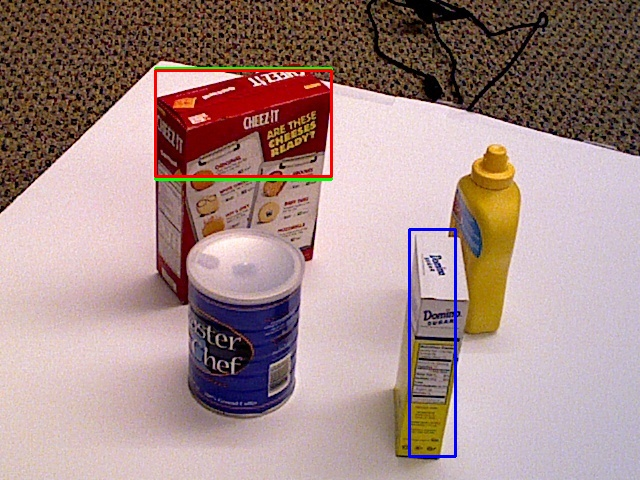
\includegraphics[width=\textwidth]{img/4_0001_000121-box.jpg}
        \caption{Detection Box for 4\_0001\_000121-box.jpg}
        \label{fig:img1}
    \end{subfigure}
    \hfill
    \begin{subfigure}{0.45\textwidth}
        \centering
        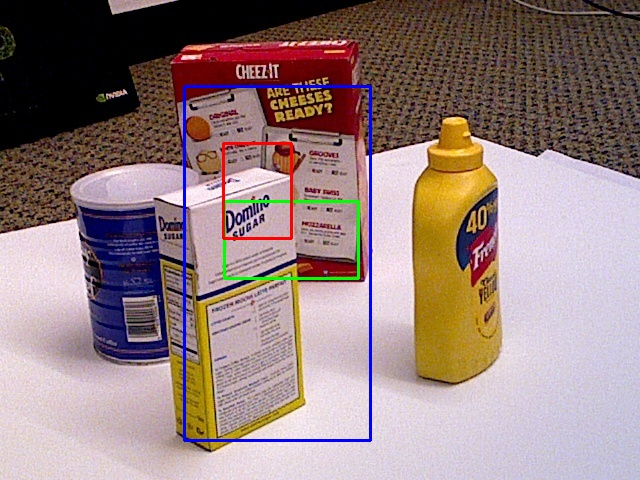
\includegraphics[width=\textwidth]{img/4_0001_000956-box.jpg}
        \caption{Detection Box for 4\_0001\_000956-box.jpg}
        \label{fig:img2}
    \end{subfigure}

    \vspace{2em}

    \begin{subfigure}{0.45\textwidth}
        \centering
        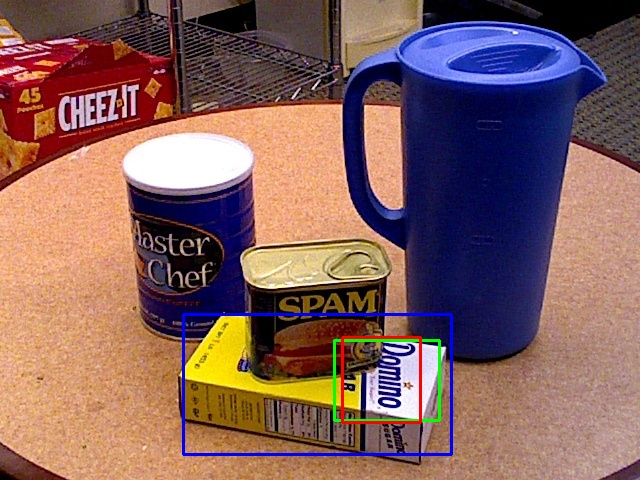
\includegraphics[width=\textwidth]{img/4_0014_001409-box.jpg}
        \caption{Detection Box for 4\_0014\_001409-box.jpg}
        \label{fig:img3}
    \end{subfigure}
    \hfill
    \begin{subfigure}{0.45\textwidth}
        \centering
        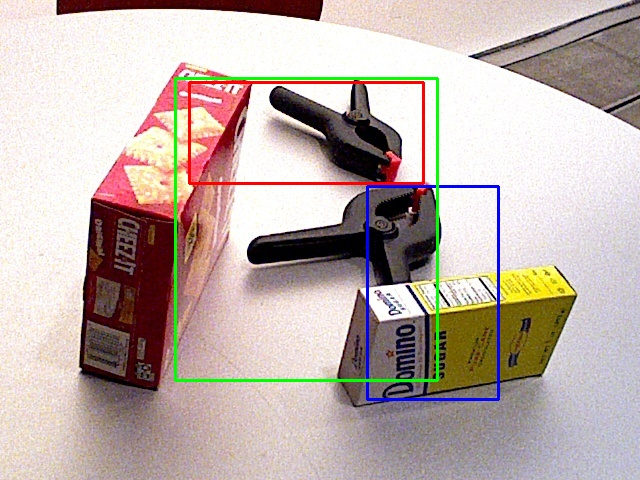
\includegraphics[width=\textwidth]{img/4_0025_000065-box.jpg}
        \caption{Detection Box for 4\_0025\_000065-box.jpg}
        \label{fig:img4}
    \end{subfigure}

    \vspace{2em}

    \begin{subfigure}{0.45\textwidth}
        \centering
        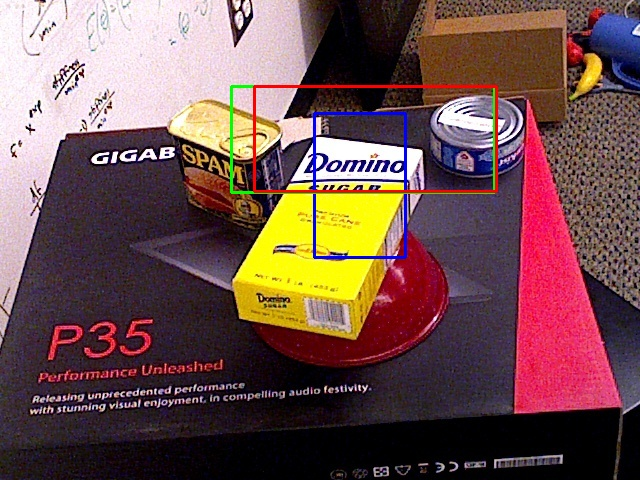
\includegraphics[width=\textwidth]{img/4_0049_000003-box.jpg}
        \caption{Detection Box for 4\_0049\_000003-box.jpg}
        \label{fig:img5}
    \end{subfigure}
    \hfill
    \begin{subfigure}{0.45\textwidth}
        \centering
        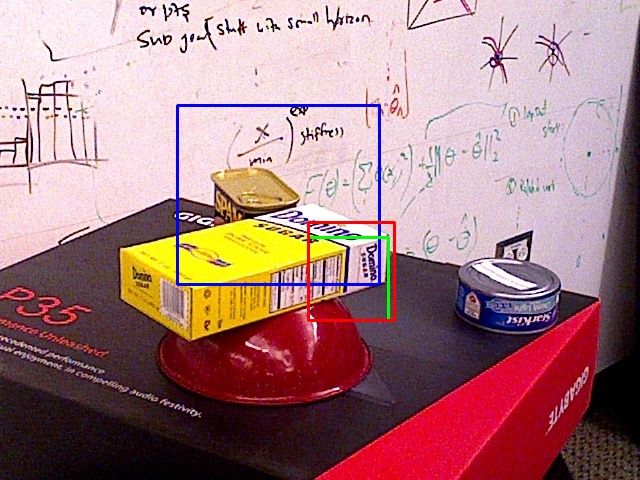
\includegraphics[width=\textwidth]{img/4_0049_000815-box.jpg}
        \caption{Detection Box for 4\_0049\_000815-box.jpg}
        \label{fig:img6}
    \end{subfigure}
    \end{figure}

    \clearpage
    \begin{figure} [h]
    \begin{subfigure}{0.45\textwidth}
        \centering
        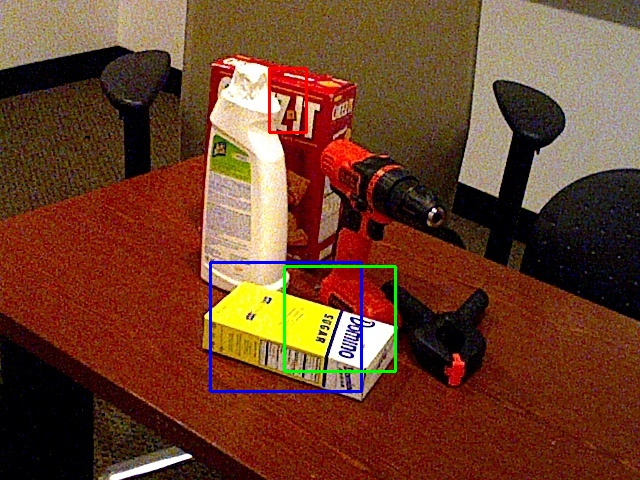
\includegraphics[width=\textwidth]{img/4_0054_000215-box.jpg}
        \caption{Detection Box for 4\_0054\_000215-box.jpg}
        \label{fig:img7}
    \end{subfigure}
    \hfill
    \begin{subfigure}{0.45\textwidth}
        \centering
        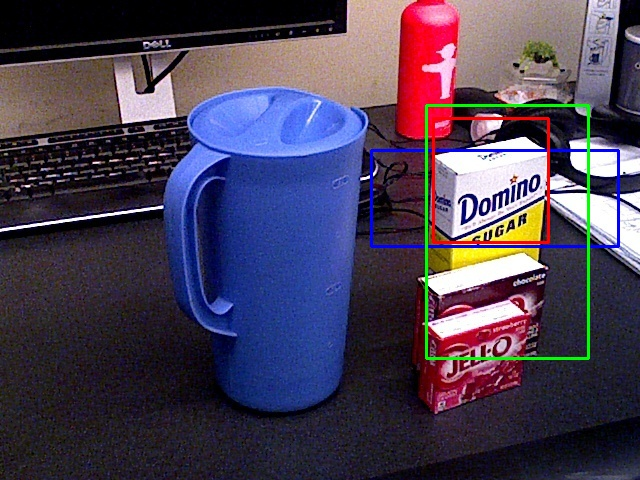
\includegraphics[width=\textwidth]{img/4_0058_000001-box.jpg}
        \caption{Detection Box for 4\_0058\_000001-box.jpg}
        \label{fig:img8}
    \end{subfigure}

    \vspace{2em}

    \begin{subfigure}{0.45\textwidth}
        \centering
        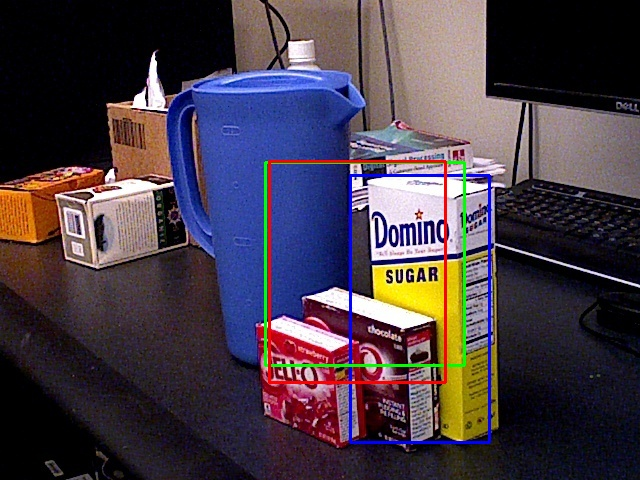
\includegraphics[width=\textwidth]{img/4_0058_001715-box.jpg}
        \caption{Detection Box for 4\_0058\_001715-box.jpg}
        \label{fig:img9}
    \end{subfigure}
    \hfill
    \begin{subfigure}{0.45\textwidth}
        \centering
        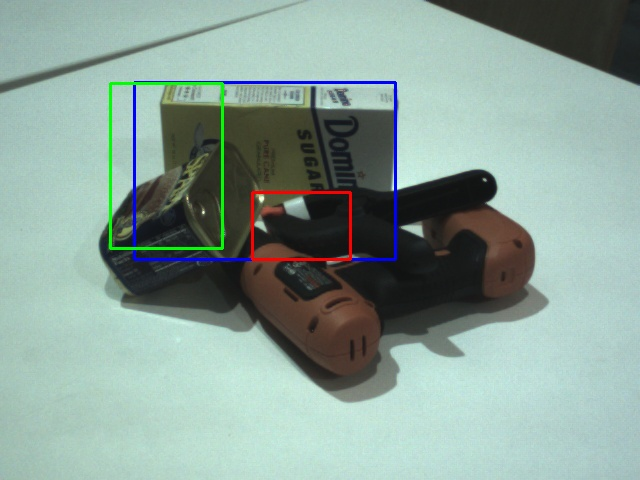
\includegraphics[width=\textwidth]{img/4_0077_000659-box.jpg}
        \caption{Detection Box for 4\_0077\_000659-box.jpg}
        \label{fig:img10}
    \end{subfigure}

    \vspace{2em}

    \begin{subfigure}{0.45\textwidth}
        \centering
        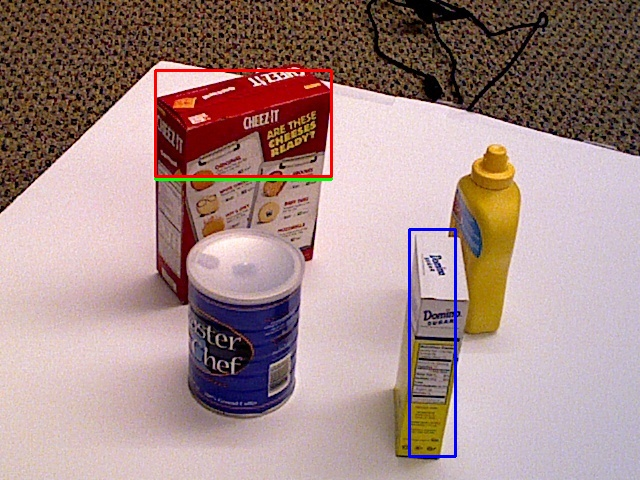
\includegraphics[width=\textwidth]{img/6_0001_000121-box.jpg}
        \caption{Detection Box for 6\_0001\_000121-box.jpg}
        \label{fig:img11}
    \end{subfigure}
    \hfill
    \begin{subfigure}{0.45\textwidth}
        \centering
        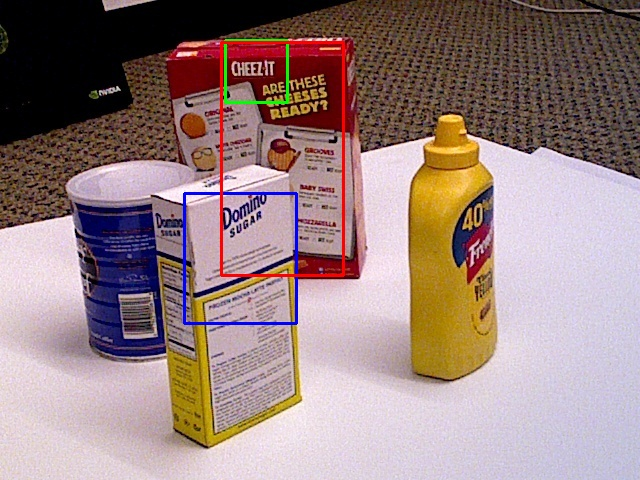
\includegraphics[width=\textwidth]{img/6_0001_000952-box.jpg}
        \caption{Detection Box for 6\_0001\_000952-box.jpg}
        \label{fig:img12}
    \end{subfigure}
    \end{figure}

    \clearpage
    
    \begin{figure}
    \begin{subfigure}{0.45\textwidth}
        \centering
        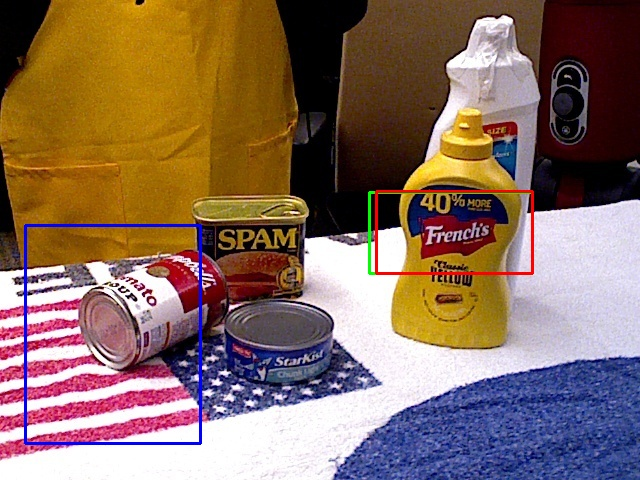
\includegraphics[width=\textwidth]{img/6_0008_001625-box.jpg}
        \caption{Detection Box for 6\_0008\_001625-box.jpg}
        \label{fig:img13}
    \end{subfigure}
    \hfill
    \begin{subfigure}{0.45\textwidth}
        \centering
        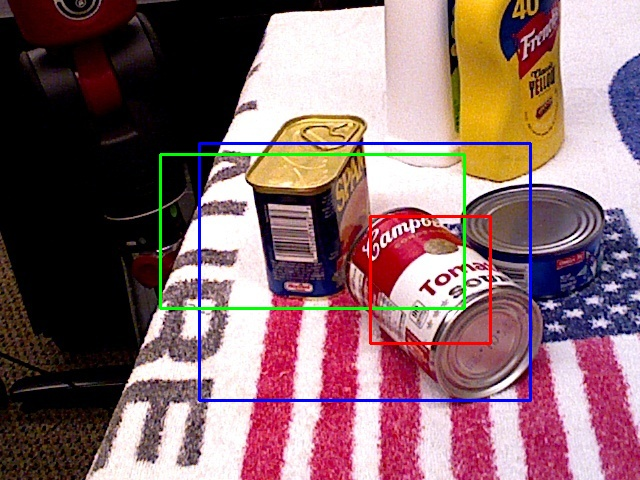
\includegraphics[width=\textwidth]{img/6_0008_002747-box.jpg}
        \caption{Detection Box for 6\_0008\_002747-box.jpg}
        \label{fig:img14}
    \end{subfigure}

    \vspace{2em}

    \begin{subfigure}{0.45\textwidth}
        \centering
        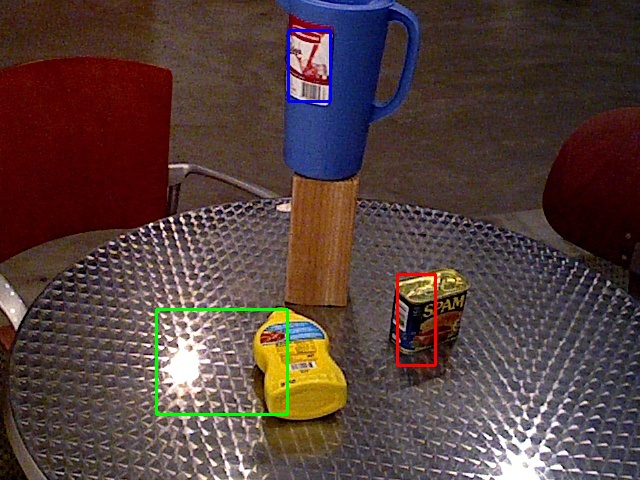
\includegraphics[width=\textwidth]{img/6_0026_000077-box.jpg}
        \caption{Detection Box for 6\_0026\_000077-box.jpg}
        \label{fig:img15}
    \end{subfigure}
    \hfill
    \begin{subfigure}{0.45\textwidth}
        \centering
        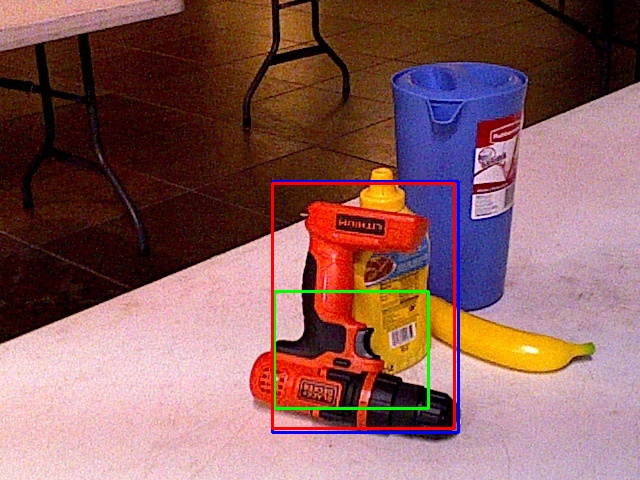
\includegraphics[width=\textwidth]{img/6_0030_000130-box.jpg}
        \caption{Detection Box for 6\_0030\_000130-box.jpg}
        \label{fig:img16}
    \end{subfigure}

    \vspace{2em}

    \begin{subfigure}{0.45\textwidth}
        \centering
        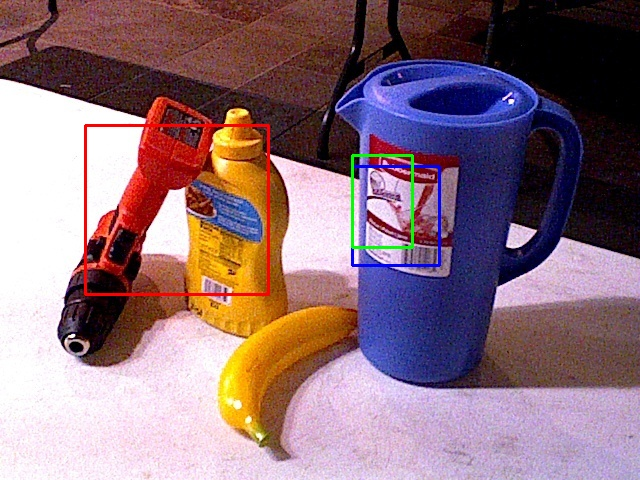
\includegraphics[width=\textwidth]{img/6_0030_001027-box.jpg}
        \caption{Detection Box for 6\_0030\_001027-box.jpg}
        \label{fig:img17}
    \end{subfigure}
    \hfill
    \begin{subfigure}{0.45\textwidth}
        \centering
        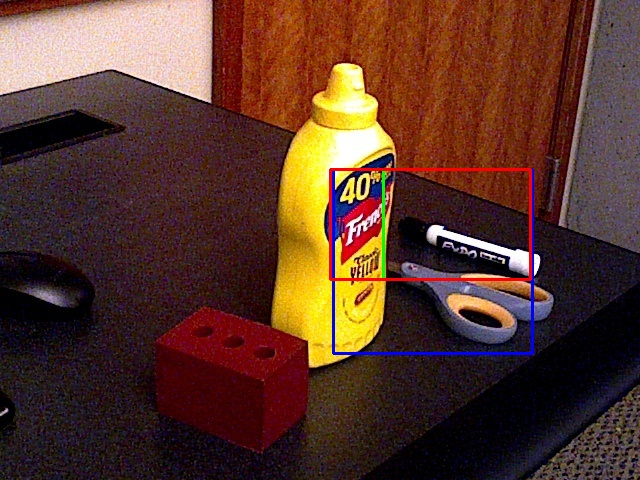
\includegraphics[width=\textwidth]{img/6_0046_000002-box.jpg}
        \caption{Detection Box for 6\_0046\_000002-box.jpg}
        \label{fig:img18}
    \end{subfigure}
    \end{figure}

    \clearpage
    
    \begin{figure}
    \begin{subfigure}{0.45\textwidth}
        \centering
        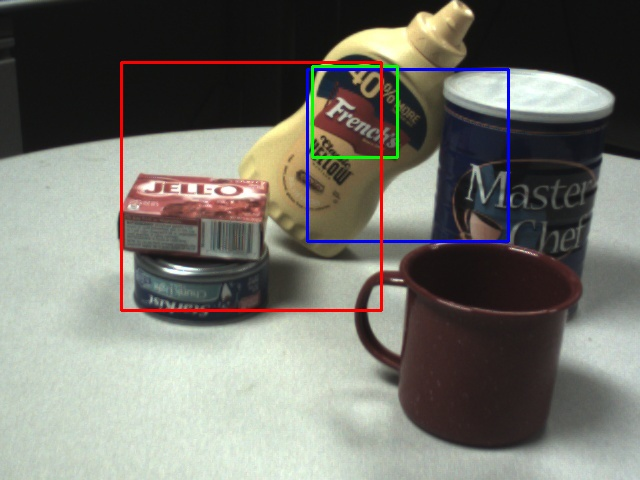
\includegraphics[width=\textwidth]{img/6_0069_000681-box.jpg}
        \caption{Detection Box for 6\_0069\_000681-box.jpg}
        \label{fig:img19}
    \end{subfigure}
    \hfill
    \begin{subfigure}{0.45\textwidth}
        \centering
        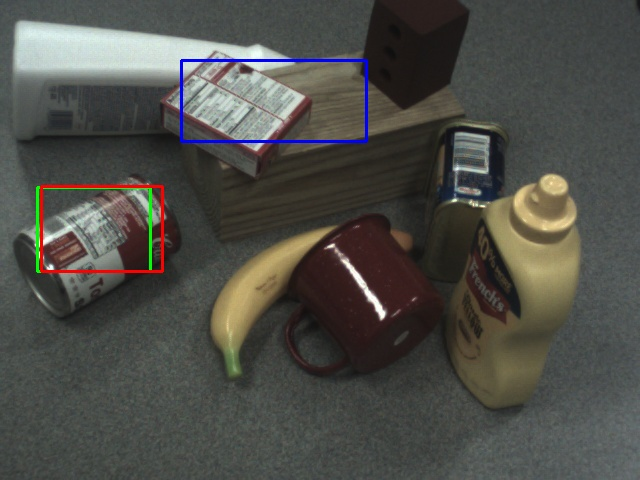
\includegraphics[width=\textwidth]{img/6_0087_000029-box.jpg}
        \caption{Detection Box for 6\_0087\_000029-box.jpg}
        \label{fig:img20}
    \end{subfigure}

    \vspace{2em}

    \begin{subfigure}{0.45\textwidth}
        \centering
        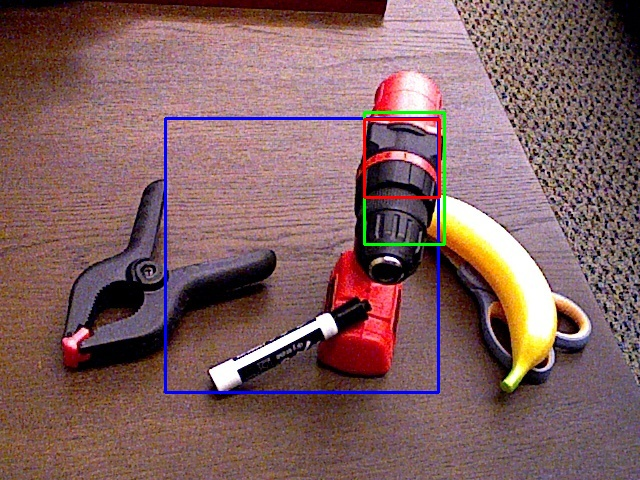
\includegraphics[width=\textwidth]{img/35_0010_000001-box.jpg}
        \caption{Detection Box for 35\_0010\_000001-box.jpg}
        \label{fig:img21}
    \end{subfigure}
    \hfill
    \begin{subfigure}{0.45\textwidth}
        \centering
        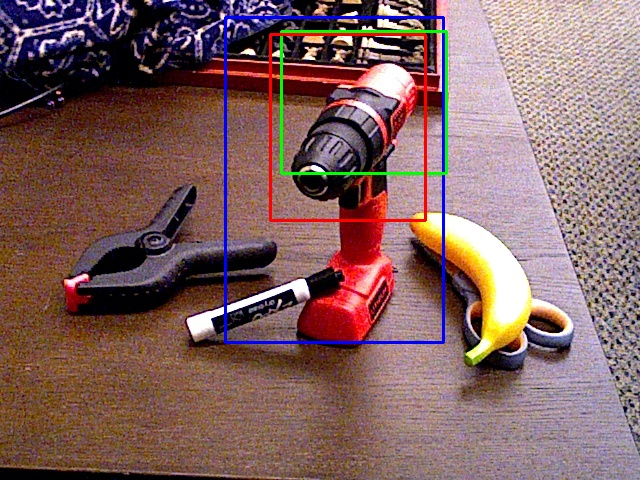
\includegraphics[width=\textwidth]{img/35_0010_000491-box.jpg}
        \caption{Detection Box for 35\_0010\_000491-box.jpg}
        \label{fig:img22}
    \end{subfigure}

    \vspace{2em}

    \begin{subfigure}{0.45\textwidth}
        \centering
        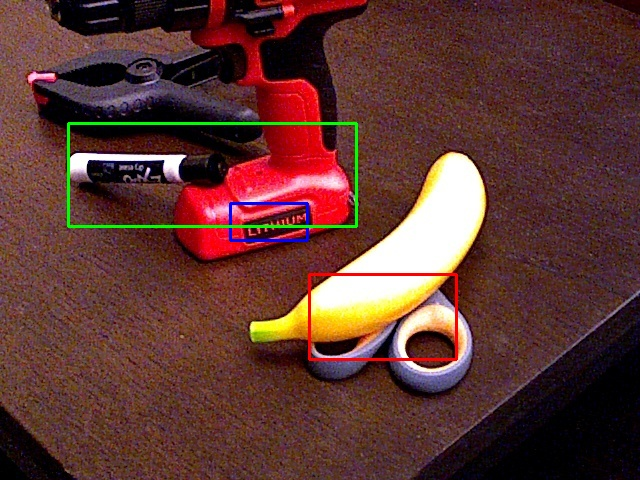
\includegraphics[width=\textwidth]{img/35_0010_000868-box.jpg}
        \caption{Detection Box for 35\_0010\_000868-box.jpg}
        \label{fig:img23}
    \end{subfigure}
    \hfill
    \begin{subfigure}{0.45\textwidth}
        \centering
        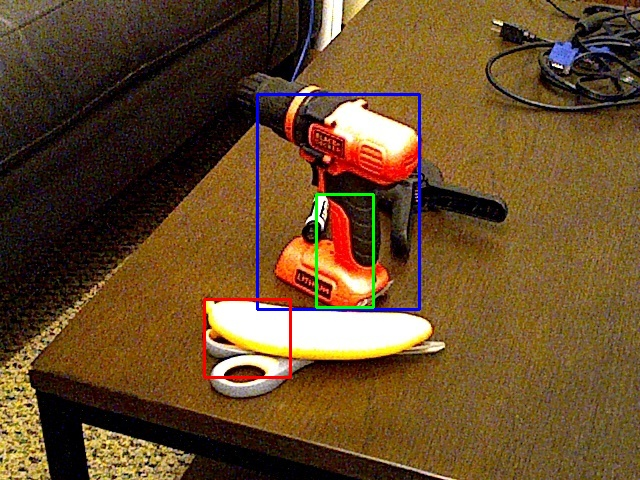
\includegraphics[width=\textwidth]{img/35_0010_001462-box.jpg}
        \caption{Detection Box for 35\_0010\_001462-box.jpg}
        \label{fig:img24}
    \end{subfigure}
    \end{figure}

    \clearpage
    
    \begin{figure}
    \begin{subfigure}{0.45\textwidth}
        \centering
        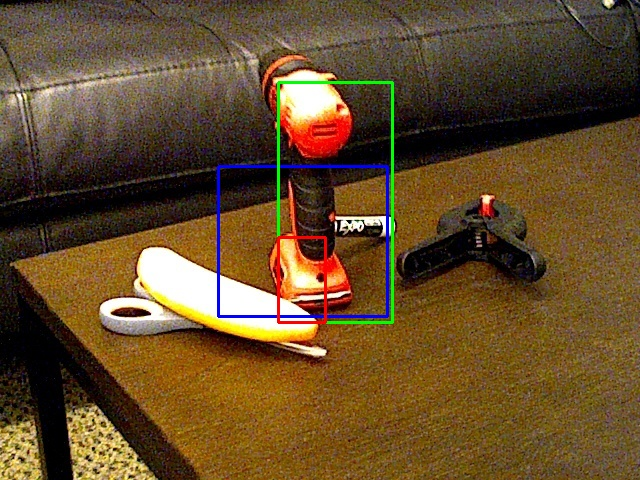
\includegraphics[width=\textwidth]{img/35_0010_001853-box.jpg}
        \caption{Detection Box for 35\_0010\_001853-box.jpg}
        \label{fig:img25}
    \end{subfigure}
    \hfill
    \begin{subfigure}{0.45\textwidth}
        \centering
        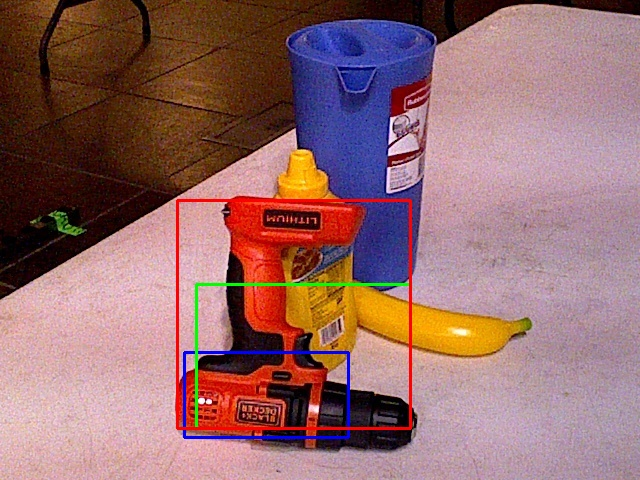
\includegraphics[width=\textwidth]{img/35_0030_000046-box.jpg}
        \caption{Detection Box for 35\_0030\_000046-box.jpg}
        \label{fig:img26}
    \end{subfigure}

    \vspace{2em}

    \begin{subfigure}{0.45\textwidth}
        \centering
        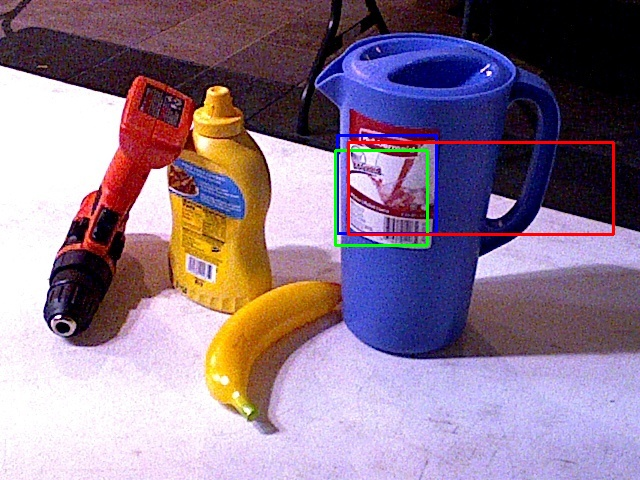
\includegraphics[width=\textwidth]{img/35_0030_001009-box.jpg}
        \caption{Detection Box for 35\_0030\_001009-box.jpg}
        \label{fig:img27}
    \end{subfigure}
    \hfill
    \begin{subfigure}{0.45\textwidth}
        \centering
        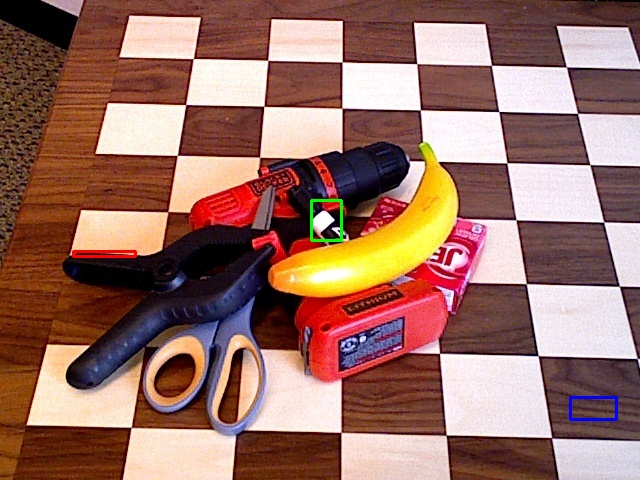
\includegraphics[width=\textwidth]{img/35_0038_002606-box.jpg}
        \caption{Detection Box for 35\_0038\_002606-box.jpg}
        \label{fig:img28}
    \end{subfigure}
    
    \vspace{2em} % Spazio verticale

    \begin{subfigure}{0.45\textwidth}
        \centering
        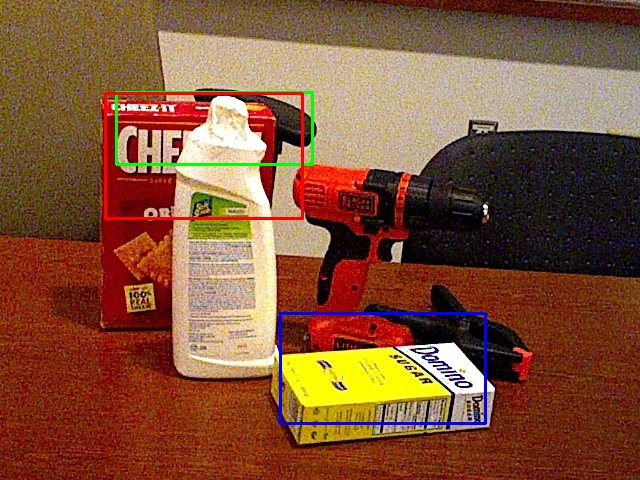
\includegraphics[width=\textwidth]{img/35_0054_001329-box.jpg}
        \caption{Detection Box for 35\_0054\_001329-box.jpg}
        \label{fig:img29}
    \end{subfigure}
    \hfill
    \begin{subfigure}{0.45\textwidth}
        \centering
        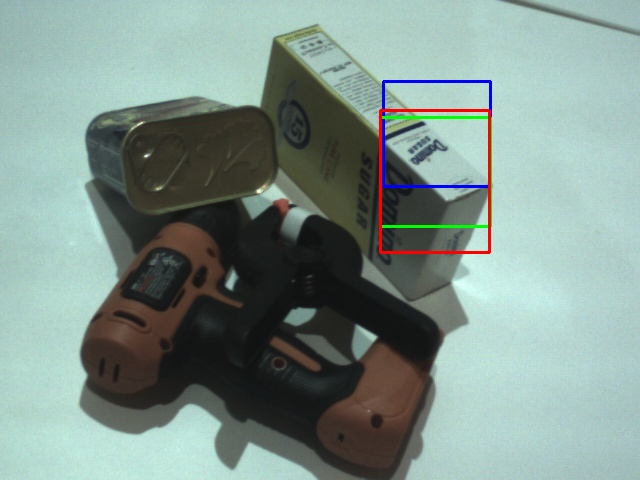
\includegraphics[width=\textwidth]{img/35_0077_000519-box.jpg}
        \caption{Detection Box for 35\_0077\_000519-box.jpg}
        \label{fig:img30}
    \end{subfigure}
\end{figure}

\begin{comment}
4_0001_000121 - 004_sugar_box -> IoU: 0.633054
4_0001_000121 - 006_mustard_bottle -> IoU: 0
4_0001_000956 - 004_sugar_box -> IoU: 0.444151
4_0001_000956 - 006_mustard_bottle -> IoU: 0
4_0014_001409 - 004_sugar_box -> IoU: 0.900687
4_0025_000065 - 004_sugar_box -> IoU: 0.397487
4_0049_000003 - 004_sugar_box -> IoU: 0.266068
4_0049_000815 - 004_sugar_box -> IoU: 0.290317
4_0054_000215 - 004_sugar_box -> IoU: 0.598793
4_0054_000215 - 035_power_drill -> IoU: 0
4_0058_000001 - 004_sugar_box -> IoU: 0.304602
4_0058_001715 - 004_sugar_box -> IoU: 0.789359
4_0077_000659 - 035_power_drill -> IoU: 0.112853
4_0077_000659 - 004_sugar_box -> IoU: 0.610422
6_0001_000121 - 004_sugar_box -> IoU: 0.633054
6_0001_000121 - 006_mustard_bottle -> IoU: 0
6_0001_000952 - 004_sugar_box -> IoU: 0.36603
6_0001_000952 - 006_mustard_bottle -> IoU: 0
6_0008_001625 - 006_mustard_bottle -> IoU: 0.31255
6_0008_002747 - 006_mustard_bottle -> IoU: 0.00472067
6_0026_000077 - 006_mustard_bottle -> IoU: 0.176487
6_0030_000130 - 006_mustard_bottle -> IoU: 0.260543
6_0030_000130 - 035_power_drill -> IoU: 0.740656
6_0030_001027 - 006_mustard_bottle -> IoU: 0
6_0030_001027 - 035_power_drill -> IoU: 0.447079
6_0046_000002 - 006_mustard_bottle -> IoU: 0.150573
6_0069_000681 - 006_mustard_bottle -> IoU: 0.135287
6_0087_000029 - 006_mustard_bottle -> IoU: 0
35_0010_000001 - 035_power_drill -> IoU: 0.165737
35_0010_000491 - 035_power_drill -> IoU: 0.435868
35_0010_000868 - 035_power_drill -> IoU: 0
35_0010_001462 - 035_power_drill -> IoU: 0.017833
35_0010_001853 - 035_power_drill -> IoU: 0.134853
35_0030_000046 - 006_mustard_bottle -> IoU: 0.245278
35_0030_000046 - 035_power_drill -> IoU: 0.827711
35_0030_001009 - 006_mustard_bottle -> IoU: 0
35_0030_001009 - 035_power_drill -> IoU: 0
35_0038_002606 - 035_power_drill -> IoU: 0
35_0054_001329 - 004_sugar_box -> IoU: 0.577564
35_0054_001329 - 035_power_drill -> IoU: 0.00911418
35_0077_000519 - 035_power_drill -> IoU: 0.0370631
35_0077_000519 - 004_sugar_box -> IoU: 0.163798
Total objects detected: 9/42
Average IoU: 0.266419
\end{comment}

\end{document}
